\section{Tune the IMM to the given data}

We initialized the filter using the values from previous excercises which we knew worked well. We then modified the \textit{simulate\_atc\_track.m} script to allow us to generate pure CV and CT tracks and used those to tune the corresponding CV/CT PDAF models, using NEES confidence interval (CI) and common sense as metrics. Multiple tracks were used for each model to increase robustness. The measurement noise $r$, clutter intensity $\lambda$, the detection probability $P_D$ and the gate size should be independent of modes, so they were tuned and balanced between the two models. The process noise for CV $q_{cv}$ and CT $q_{ct}$ were tuned individually using their correspondig models. For IMM PDAF tuning we created a custom plot function which allowed us to plot the tracked path in colors corresponding to the mode probability (see fig \ref{fig:task22_modeprob}). We then tuned the IMM Markov Matrix $PI$ so that the CV model was used during constant velocity sections of the track, and the CT models during the turns (fig \ref{fig:task22_modeprob_tuned}). $q_{cv}$ and $q_{ct}$ does affect the mode probabilities, i.e we risk always prefering one model if the process noises are not balanced (see fig \ref{fig:task22_modeprob_highcv} where $q_{cv}$ is big compared to $q_{ct}$). Our finished tuning \ref{eq:tuning} works well and seems to balance the two models well.
\begin{subequations} \label{eq:tuning}
    \begin{equation}
        r = 5
    \end{equation}
    \begin{equation}
        \lambda = 10^{-4} 
    \end{equation}
    \begin{equation}
        P_D = 0.95
    \end{equation}
    \begin{equation}
        \texttt{gateSize} = 5^2 
    \end{equation}
    \begin{equation}
        q_{cv} = 0.0078 
    \end{equation}
    \begin{equation}
        q_{ct} = \begin{bmatrix}0.02 & 0.0005\end{bmatrix}
    \end{equation}
    \begin{equation}
        PI = \begin{bmatrix}0.90 & 0.05 \\ 0.10 & 0.95\end{bmatrix}
    \end{equation}
\end{subequations}

\begin{figure}
    \centering
    \hspace{-3cm}\begin{adjustbox}{minipage=\linewidth, scale=1.3}
        \begin{subfigure}{.5\textwidth}
            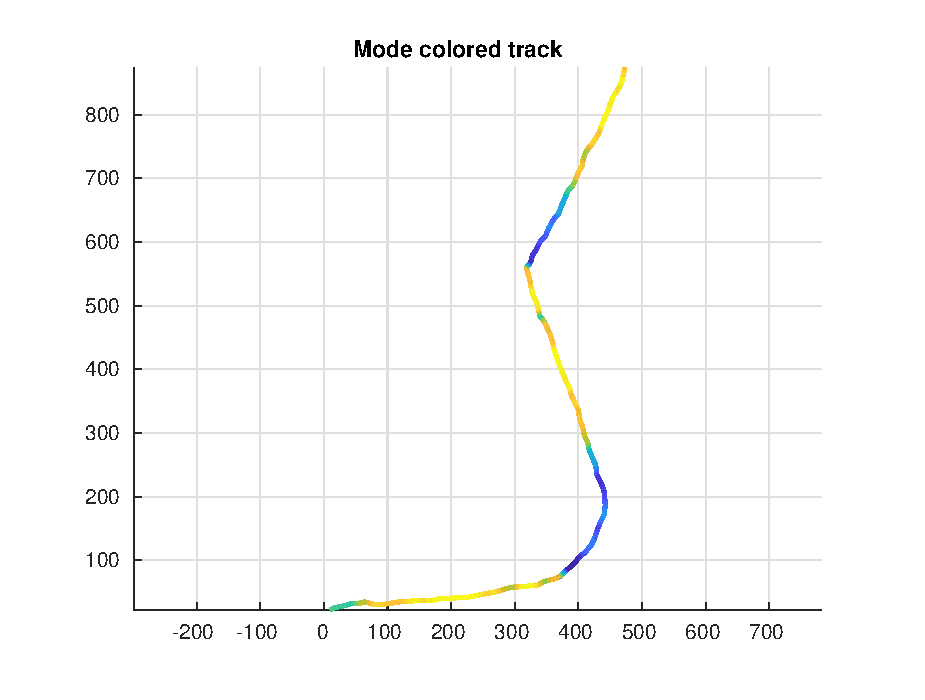
\includegraphics[width=\linewidth]{plots/task22_modeprob.eps} 
            \caption{Our tuning}
            \label{fig:task22_modeprob_tuned}
        \end{subfigure}
        \begin{subfigure}{.5\textwidth}
            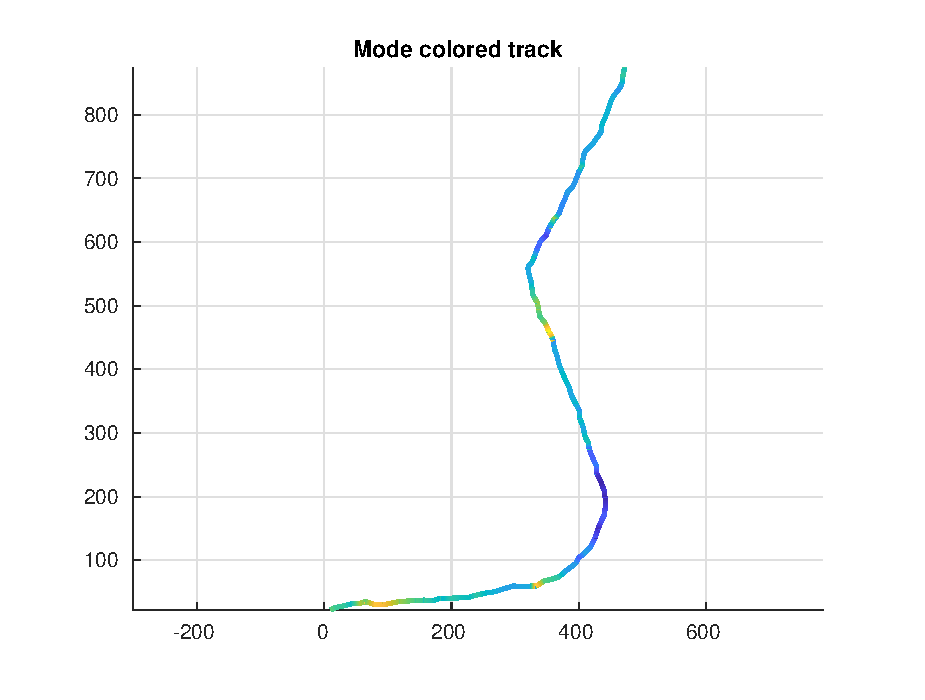
\includegraphics[width=\linewidth]{plots/task22_modeprob_highcv.eps} 
            \caption{$q_{cv}$ and $q_{ct}$ not in balance}
            \label{fig:task22_modeprob_highcv}
        \end{subfigure}
    \end{adjustbox}
        \caption{Mode probability plot: Yellow = CV, Blue = CT}
        \label{fig:task22_modeprob}
\end{figure}
